\section{Entwicklungsansätze mobiler Anwendungen}
\label{sec:Entwicklungsansaetze}
Bei der Entwicklung von Anwendungen für Mobilgeräte wird meist zwischen den drei grundlegenden Ansätzen \textit{Native}, \textit{Hybrid} und \textit{Web} unterschieden \cite{Nunkesser_Taxonomy_Apps, Que_Comparison_Hybrid_Native}.
Die native Entwicklung beschreibt dabei die Anwendungsentwicklung spezifisch für ein bestimmtes Betriebssystem mit den \acp{SDK} und Programmiersprachen, die der Betriebssystemhersteller für die Entwicklung bereitstellt.
Für iOS sind das die Programmiersprachen Objective-C und Swift.
Bei Android kommen Java und Kotlin zum Einsatz.
Sollen beide Betriebssysteme unterstützt werden, muss bei diesem Ansatz die Anwendung für jedes System in einer der entsprechenden Sprachen gesondert entwickelt werden.
Für die Entwicklung wird dementsprechend ein Team mit Kenntnissen in beiden Systemen oder getrennte Entwicklungsteams pro Plattform benötigt.
Das hat nicht nur Auswirkungen auf die Entwicklungskosten, sondern auch auf die Geschwindigkeit der Entwicklung \cite{Manchanda_CrossPlatformFrameworks}.
Dennoch wird dieser Ansatz häufig eingesetzt, um die größtmögliche Performance zu erhalten und auf alle vom Betriebssystem zur Verfügung gestellten \acp{API} zugreifen zu können \cite{Pinto_Native_to_Cross_Platform}.

Beim Web-Ansatz hingegen, wird eine Webanwendung entwickelt, die komplett im Browser und damit unabhängig vom Betriebssystem lauffähig ist.
Hierzu werden klassischerweise \ac{HTML}, \ac{CSS} und JavaScript verwendet.
Der hybride Ansatz versucht beide Ansätze zu kombinieren, indem Webanwendungen in native Anwendungen eingebettet werden.
Somit können teilweise native Funktionen wie Smartphone-Sensoren und spezielle \acp{API} verwendet werden, während die Anwendung in einem eingebetteten Browser läuft und überwiegend mit Web-Technologien entwickelt werden kann \cite{Nunkesser_Taxonomy_Apps}.

Die Ansätze Hybrid und Web ermöglichen die Wiederverwendung von Code zwischen den verschiedenen Plattformen.
Demnach können beide Ansatz unter dem Überbegriff Cross-Plattform zusammengefasst werden.
Allerdings bieten Web-Apps nur sehr geringen Zugriff auf die Hardware des Geräts und können daher nicht alle Anwendungsfälle abdecken.
Außerdem lassen sie sich nicht über die App-Stores der Betriebssysteme verteilen.
Deshalb wird der Web-Ansatz für die Zwecke dieser Arbeit nicht zu den Cross-Plattform-Ansätzen gezählt.
Im Folgenden soll die Bezeichnung Cross-Plattform, jeweils als ein Ansatz verstanden werden, der die Wiederverwendung von Code, insbesondere zwischen den beiden mobilen Plattformen Android und iOS, fördert.
Außerdem müssen Apps lokal installiert und über die App-Stores der Betriebssysteme verteilt werden können.
Gefordert wird zusätzlich die Möglichkeit, auf native Gerätefunktionen, wie Gerätesensoren oder die Kamera, zuzugreifen.
Es wird für die Kategorisierung nicht gefordert, dass der komplette Code wiederverwendet werden kann.

Inzwischen gibt es eine Vielzahl von Frameworks, welche diese Kriterien erfüllen, aber nicht dem hybriden Ansatz zugeordnet werden können.
Deshalb führt Nunkesser in \cite{Nunkesser_Taxonomy_Apps} eine feinere Unterteilung der Entwicklungsansätze auf Basis der verwendeten Tools und Technologien ein.
Die Unterteilung in sechs Kategorien und ihre wichtigsten Merkmale ist in der Tabelle in \ref{tab:Taxonomy_Nunkesser} dargestellt.
Außerdem ist in der letzten Spalte angegeben, ob die App-Kategorie die plattformübergreifende Wiederverwendung von Code unterstützt.
\begin{table}[H]
    \begin{tabularx}{\textwidth}{ |l|X|r| }
        \hline
        \textbf{Kategorie}      & \textbf{Kennzeichen}  & \textbf{Plattformübergreifende} \\ & & \textbf{Code-Wiederverwendung}                                                   \\
        \Xhline{0.5mm}
        \hline
        Endemic Apps            & Verwendung Plattformspezifischer Tools, \acp{SDK} und Programmiersprachen bereitgestellt vom Betriebssystemhersteller, Kompilation, Teilweise \ac{JIT}-Kompilation möglich                        & \xmark        \\
        \hline
        Web-Apps                & Verwendung von Web-Technologien, Interpretation im Browser des Zielgeräts                                                                                                                         & \cmark        \\
        \hline
        Hybrid Web-Apps         & Verwendung von Web-Technologien, eingebettet in eine Endemic App, Kombination von kompilierten und interpretierten Teilen                                                                         & \cmark        \\
        \hline
        Hybrid Bridged Apps     & Erweiterung von Hybrid Web-Apps um \ac{UI} Elemente von Endemic Apps, Kombination von kompilierten und interpretierten Teilen                                                                     & \cmark        \\
        \hline
        System Language Apps    & Verwendung von Low-Level Programmiersprachen wie C/C++ und Plattformspezifische Kompilation                                                                                                       & (\xmark)      \\
        \hline
        Foreign Language Apps   & Verwendung von Programmiersprachen, die vom Betriebssystemhersteller nicht für Endemic Apps vorgesehen sind, in der Regel Kompilation, Teilweise \ac{JIT}-Kompilation und Interpretation möglich   & \cmark       \\
        \hline
    \end{tabularx}
    \caption{App-Kategorien und Entwicklungsansätze nach Nunkesser \cite{Nunkesser_Taxonomy_Apps}}
    \label{tab:Taxonomy_Nunkesser}
\end{table}

Eine wichtige Neuerung ist die Einführung der neuen Kategorie der \textit{Foreign Language Apps}, welche keiner anderen Kategorie untergeordnet werden können.
Populäre Frameworks wie Xamarin und Flutter gehören zur Kategorie der Foreign Language Apps und ermöglichen die Entwicklung mit C\# respektive Dart, welche weder von Android noch von iOS für die Entwicklung von Apps vorgesehen sind \cite{Xamarin_Homepage,Flutter_Architektur}.
Weiterhin differenziert er den Hybrid Ansatz weiter und führt die Endemic Apps, abgeleitet aus dem griechischen, als neue Bezeichnung für den nativen Ansatz ein.
Alle nicht den Endemic Apps zugeordneten Ansätze nennt er als Gegensatz zu Endemic Apps, Ecdemic Apps.
Pandemic Apps ist der Überbegriff für alle Apps, welche auf Sprachen setzen die auf beiden Systemen verfügbar sind, wie zum Beispiel C/C++ oder JavaScript \cite{Nunkesser_Taxonomy_Apps}.
Pandemic und Ecdemic dienen vor allem zur Sammlung verwandter Ansätze, werden im Folgenden allerdings nicht weiter verwendet.
Nunkessers Taxonomie bietet allerdings auch Bezeichnungen für die einzelnen Ansätze, die das Grundkonzept des jeweiligen Ansatzes einfach verständlich machen.
Deshalb werden die von ihm eingeführten Bezeichnungen im Folgenden verwendet.

Für den Zweck dieser Arbeit wird in den folgenden Abschnitten vorwiegend die übergreifende Kategorie Cross-Plattform verwendet.
Diese umfasst die \textit{Hybrid Web Apps}, \textit{Hybrid Bridged Apps} und Foreign Language Apps.
Die zu untersuchenden Frameworks werden jeweils in eine der Unterkategorien eingeordnet, um Vergleiche zwischen diesen besser zu ermöglichen.
Die von Nunkesser als \textit{System Language Apps} bezeichnete Kategorie wird im Rahmen dieser Arbeit nicht als Cross-Plattform angesehen.
Bei System Language Apps erfolgt eine starke Bindung an das jeweilige \ac{SDK}, was die Wiederverwendung von Code sehr schwierig macht.
Bei geeigneter Architektur der App ist es hier jedoch möglich, Teile des Codes Systemübergreifend zu verwenden.
Für die Untersuchung von Frameworks für die Plattformübergreifende Entwicklung spielt dieser Ansatz aufgrund fehlender populärer Frameworks keine Rolle.
Außerdem ist die Bedeutung dieses Ansatzes für die Entwicklung mobiler Anwendungen in der Praxis allgemein vergleichsweise gering \cite{Nunkesser_Taxonomy_Apps}.


\subsection{Allgemeine Vor- und Nachteile von Cross-Plattform Entwicklung}
\label{sec:CrossPlattform_Vorteile}

Die wichtigsten allgemeinen Vorteile und Nachteile der Cross-Plattform Entwicklung im Vergleich zur nativen Entwicklung, laut Manchanda \cite{Manchanda_CrossPlatformFrameworks} sind in \autoref{fig:Native_vs_CrossPlatform} tabellarisch aufgeführt.
\begin{figure}[H]
    \centering
    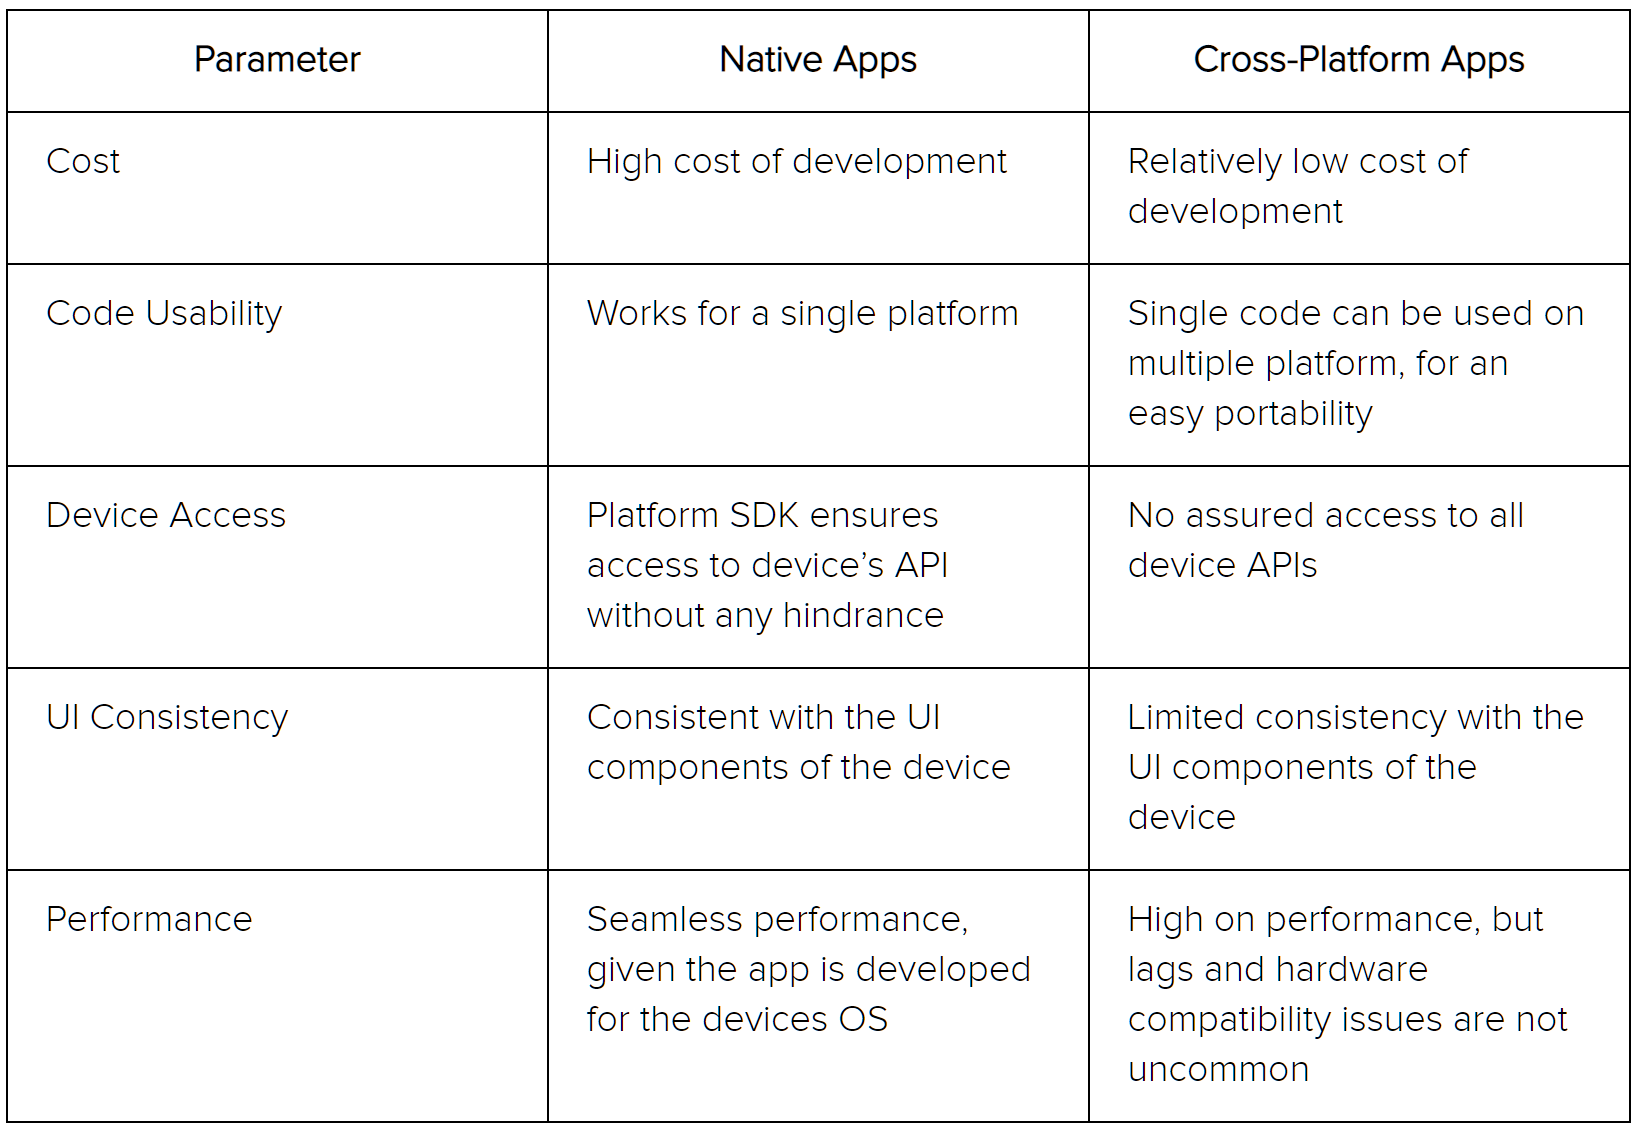
\includegraphics[width=0.9\textwidth]{Native_vs_CrossPlatform.png}
    \caption{Gegenüberstellung Entwicklungsansätze Native und Cross-Plattform \cite{Manchanda_CrossPlatformFrameworks}.}
    \label{fig:Native_vs_CrossPlatform}
\end{figure}

Alle Ansätze der teilen sich den Vorteil eines reduzierten Entwicklungsaufwands und verringerter Kosten durch die einfache Wiederverwendung von Code.
Je nach verwendetem Framework kann der Anteil des geteilten Codes bis zu 100 \% betragen \cite{NET_MAUI_Introduction,Nawrocki_Comparison_Hybrid_Native_Frameworks}.
Generell zeichnen sich diese Frameworks dadurch aus, dass der überwiegende Teil des Codes wiederverwendet werden kann \cite{Nawrocki_Comparison_Hybrid_Native_Frameworks}.
Matt Kremer, Enterprise Product Manager für das Ionic-Framework, demonstiert mit einem Beispiel, dass die Kosten für eine Ionic-basierte App weniger als 30 \% der Kosten einer vergleichbaren nativen App betragen können \cite{Kremer_IonicROI}.
Hier ist jedoch zu bedenken, dass diese Angaben nicht durch eine unabhängige Quelle bestätigt wurden.
Allgemein sind sich sowohl Framework-Anbieter \cite{Xamarin_Homepage, Kremer_IonicROI} als auch unabhängige Wissenschaftler \cite{Pinto_Native_to_Cross_Platform, Que_Comparison_Hybrid_Native, Nawrocki_Comparison_Hybrid_Native_Frameworks} einig, dass eine Cross-Plattform Entwicklung deutliche Kostenvorteile mit sich bringt.

Probleme gibt es im Vergleich zur nativen Entwicklung beim Zugriff auf native \acp{API} der Geräte.
Einige Frameworks bieten direkten Zugriff auf einige \acp{API}, andere setzen für jeglichen Zugriff auf ein Plugin-System \cite{Heitkoetter_CrossPlatform_Comparison, Sasidaran_Survey_NativeHybrid}.
Meist können in einer Cross-Plattform App jedoch nicht alle nativ zur Verfügung stehenden Schnittstellen verwendet werden \cite{Pinto_Native_to_Cross_Platform}.

Auch bei der Konsistenz der Benutzeroberflächen schneiden die Cross-Plattform Ansätze meist schlechter \cite{Manchanda_CrossPlatformFrameworks}.
Allerdings gibt es hier starke Unterschiede zwischen den Frameworks. 
Zum Beispiel verwendet React Native jeweils native \ac{UI}-Elemente, sodass die Benutzeroberfläche dem Look-and-Feel der Plattform entsprechen kann \cite{Cook_ReactNativeBridge}.
Außerdem legen immer mehr Frameworks großen Wert auf die \ac{UI} wie sich an verschiedenen Tools für die \ac{UI}-Entwicklung zeigt \cite{NET_MAUI_Introduction,Flutter_Architektur}

Ein weiterer gemeinsamer Nachteil aller Cross-Plattform Ansätze ist die durchschnittlich geringere Performance im Vergleich zu nativen Anwendungen \cite{Que_Comparison_Hybrid_Native, Pinto_Native_to_Cross_Platform}.
Allgemein ist die Bewertung der Performance eines Frameworks immer vom Anwendungsfall und den konkret verwendeten Performancemetriken abhängig.
In der Literatur finden sich verschiedene Untersuchungen \cite{Nawrocki_Comparison_Hybrid_Native_Frameworks,Biorn-Hansen_PerformanceOverhead_CrossPlatform}, welche sich mit der Performance von verschiedenen Cross-Plattform Frameworks in verschiedenen Anwendungsfällen beschäftigen.
In keiner dieser Arbeiten wird jedoch die Performance für den konkreten Anwendungsfall der Videoaufzeichnung ausführlich untersucht.
Weiterhin gibt es keine Untersuchung, welche die Performance aller in dieser Arbeit untersuchten Frameworks miteinander vergleicht.